\documentclass[12pt,letterpaper]{article}
\usepackage{amsmath,amsfonts,amssymb}
\usepackage[margin=1in]{geometry}
\usepackage{setspace}
\usepackage{fancyhdr}
\usepackage{titlesec}
\usepackage{hyperref}
\usepackage{graphicx}
\usepackage{listings}
\usepackage{xcolor}
\usepackage{booktabs}
\usepackage{array}
\usepackage{float}
\usepackage{enumitem}

\onehalfspacing

\pagestyle{fancy}
\fancyhf{}
\lhead{Module 3 Project: Statistical Foundations of the Volatility Model}
\rhead{\thepage}

\hypersetup{colorlinks=true, linkcolor=blue, urlcolor=blue}

\title{Statistical Foundations of the Volatility Term Structure Model \\
       \large COMP 653 Statistical Machine Learning, Summer 2026}
\author{}
\date{}

\begin{document}
\maketitle

\begin{abstract}
We study whether the future movement of a stock can be predicted, and we find
that its direction is close to a coin flip while its volatility is strongly
predictable because volatility clusters in time. We therefore predict the
volatility of a stock as a function of the time horizon, from five minutes to one
hundred eighty days, and we express the forecast as a calibrated range of future
prices rather than a single number. The model runs six window LSTM branches
linked by their drift and coupled into a smooth term structure, trained jointly
with quantile heads that produce conformally calibrated price bands, and it is
combined with a cross sectional network of complementary branches under a softmax
meta layer. On out of sample data the direction target sits near an area under
the curve of one half, while the volatility term structure rises with the horizon
and reaches about $0.92$ intraday and $0.88$ daily, and the price bands cover
their nominal ninety percent rate. We give the full derivation of every function
the model uses, from the branch gradients and backpropagation through time to the
pinball loss, the conformal coverage bound, and the ensemble, and we illustrate
each with worked numbers and charts so the statistics and the software describe
the same model.
\end{abstract}

\tableofcontents
\clearpage

\section{Problem Definition}

The abstract stated the result in words. Here we make the problem precise and
give the definitions the rest of the paper builds on. The following subsections
state the concrete goal, the formal target as a conditional volatility, the
statistical reason the signal exists, the term structure across horizons, and the
way the volatility forecast becomes a range of future prices.

\subsection{The Project Goal}

Our goal is stated in one sentence. Given a stock, a target price, and a time
horizon, we predict how far the price will move and we report the probability
that it reaches the target by a target date, together with the full range of
prices the stock can reach at each horizon.

The most ambitious form of this goal is a fully specified claim about a single
name. We would like to say that stock $X$ reaches price $Y$ by date $D$ at time
$T$, then holds above a level $P$, and delivers a total gain of $M$ dollars on a
position. We treat that sentence as the target the project aims at, and we build
every component toward answering it.

Markets are close to efficient in direction, so we cannot promise a single
deterministic path to that claim, and it would be dishonest to pretend
otherwise. What we can deliver is the honest probabilistic version of the same
statement. For the event that stock $X$ trades at or above price $P$ by date $D$
we estimate
\[
\boxed{\ \widehat{\Pr}\bigl(P_{X, D} \ge P \ \big|\ \mathcal{F}_t\bigr),\ }
\]
and we surround it with a calibrated price cone whose width is set by the
predicted volatility, so the target price, the date, and the level all read off
one forecast. A wider cone means a larger span of possible gain $M$, and a
tighter cone means a more confident claim. In this way the ultra specific goal
becomes a probability and an interval that we can measure and trust, rather than
a certainty that no model can provide.

\subsection{What Is Being Predicted}

We write $\mathcal{F}_t$ for the information available at time $t$, which is every
price, return, and feature up to and including day $t$. Over the next $h$ trading
days the stock earns a cumulative log return, and the object we predict is the
conditional volatility of that return, which is the standard deviation of the
future path given what is known today,
\[
\sigma_{t,h} = \sqrt{\operatorname{Var}\!\left(\sum_{k=1}^{h} r_{t+k}
\ \middle|\ \mathcal{F}_t\right)} .
\]

The reason we target the conditional volatility rather than the raw return is a
basic fact about markets. The expected next return given the past is close to
zero, which is the efficient market statement that the sign of a move is almost
a coin flip,
\[
\mathbb{E}\!\left[\,r_{t+1} \mid \mathcal{F}_t\,\right] \approx 0 .
\]

Because the mean is unpredictable the direction carries almost no signal, and in
the experiments the direction classifier scores an area under the curve near one
half. The magnitude of the move is a different story, and that is where the
signal lives.

\subsection{Why Volatility Clusters in Time}

Volatility is predictable because large moves follow large moves and calm
follows calm, which is the property called volatility clustering. Stated in
statistics, the squared returns are positively autocorrelated and that
autocorrelation decays only slowly, so today's turbulence forecasts tomorrow's,
\[
\operatorname{Corr}\!\left(r_t^2,\, r_{t-k}^2\right) > 0
\quad\text{for many lags } k .
\]

This persistence is intrinsic to how information and trading arrive in clusters,
and it means the conditional variance is a smooth and slowly changing process
rather than noise. That is exactly the property a learner can exploit, so the
volatility label provides a clear tone for the training signal while the
direction label does not. The measured contrast is stark, with the direction
target near an area under the curve of one half and the volatility target near
one.

\subsection{The Horizon and the Term Structure}

Predicting with respect to time means predicting at many horizons at once. The
conditional volatility depends on how far ahead we look, and the collection of
these values across horizons is the volatility term structure,
\[
h \ \longmapsto\ \sigma_{t,h},
\qquad h \in \{1, 5, 10, 30, 90, 180\}\ \text{days} .
\]

Because volatility clusters, longer horizons average over more of the persistent
component and become steadier and more predictable, which is why the area under
the curve rises with the horizon in the results. The model reads six time
windows in parallel and couples their predictions into one smooth curve, so it
learns the whole term structure rather than a single horizon in isolation.

\subsection{From Volatility to a Range of Gains and Losses}

Although volatility does not tell us the sign of the next move, it tells us how
wide the range of outcomes is, which is what a trader cares about when sizing a
position. We turn the predicted volatility into an explicit range of future
prices by learning quantiles of the return, so the model reports a cone of
possible gains and losses whose width is set by the predicted volatility. A wider
cone means a more volatile stock and a larger span of possible gain or loss,
which is the practical reading of the forecast.

In short the problem is to forecast, at each horizon, how volatile a stock will
be relative to its peers, to exploit the fact that volatility clusters in time,
and to express the forecast as a calibrated range of future gains and losses.

\clearpage
\section{Solution Design and Key Features}

Our design solves the problem by attacking it at every scale of time at once,
by learning the target with a set of complementary models, and by turning the
forecast into a calibrated range rather than a single number. This section walks
through the design and maps each choice to the part of the problem it answers,
and the sections that follow derive the formulas behind each piece. The whole
pipeline is shown in Figure \ref{fig:arch}.

\begin{figure}[H]
\centering
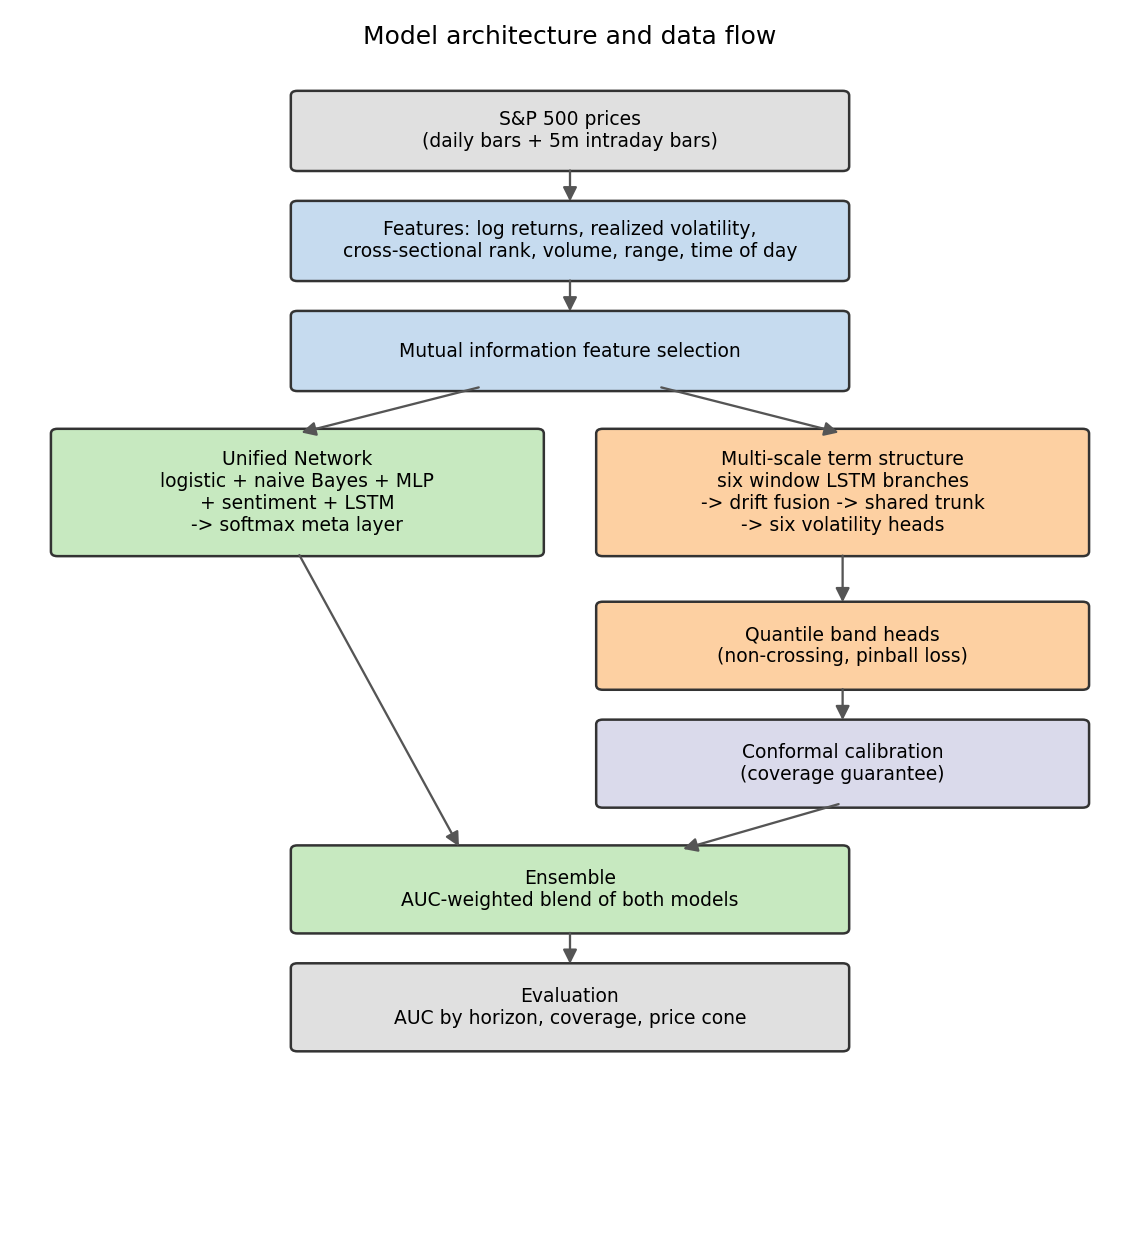
\includegraphics[width=0.74\textwidth]{figures/derivations/architecture.png}
\caption{The data flow from raw prices to the calibrated forecast. Features feed
a mutual information filter, then two complementary models, then conformal
calibration and an ensemble, and finally the horizon by horizon evaluation.}
\label{fig:arch}
\end{figure}

\subsection{Target Choice That Matches the Signal}

The first design decision is to predict volatility rather than direction, because
the problem analysis showed that the sign of a move is near a coin flip while the
size of a move clusters in time. We make the target market neutral by ranking each
stock against its peers on the same date and splitting at the median, so the
model learns relative volatility and does not simply detect whether the whole
market is calm. The exact label is derived in Section 3.

\subsection{Multi Scale Term Structure With Drift}

Because volatility is predicted with respect to time, the design reads six time
windows in parallel, one for each horizon of one, five, ten, thirty, ninety, and
one hundred eighty days. Each window is a recurrent branch that summarizes what
that scale sees, and the branches are linked by their drift, the difference
between adjacent scale embeddings, which measures how the short view departs from
the long view. The drift is part of the forward pass, so its gradient trains
every branch, and a curvature penalty keeps the six horizon predictions on one
smooth term structure. This is the core feature that lets one model learn the
whole curve rather than a single horizon, and its formulas are in Section 11.

\subsection{Complementary Models Under One Roof}

No single learner captures every pattern, so the design combines several. The
unified network runs a logistic branch, a Gaussian naive Bayes branch, a
rectified network, a sentiment branch, and a recurrent branch, then a softmax
meta layer learns how much to trust each. The linear branches capture simple
monotone effects, the rectified network captures interactions, and the recurrent
branch captures the recent path. Each branch is derived in Sections 4 through 9.

\subsection{A Calibrated Range of Prices, Not a Point}

The forecast is only useful if it states how wide the range of outcomes is, so
the design adds quantile heads that predict a band of future returns at each
horizon. The band is built to be monotone so its edges never cross, it is trained
with the pinball loss that targets a chosen quantile, and it is wrapped in
conformal calibration so the band covers its nominal rate out of sample with a
finite sample guarantee. Turning the return band into prices produces the cone of
possible gains and losses. These pieces are derived in Sections 12 and 13.

\subsection{Robust Training and Honest Evaluation}

The design trains every weight with Adam and standardizes features on training
rows only, so the test period never leaks into the scaler. It selects features by
mutual information to shrink the input, and it judges every horizon by the area
under the ROC curve, which measures ranking quality and ignores the threshold.
Finally an ensemble blends the two models by the weight that maximizes validation
area under the curve. The optimizer, the metric, and the ensemble are derived in
Sections 10, 15, and 16.

With the design and its key features in view, the remaining sections build each
formula from first principles and work real numbers through it.

\clearpage
\section{The Model Lifecycle from Data to Tuning}

Before the formulas we give the high level view of how the model actually runs
end to end, because the mathematics only makes sense inside this loop. The full
lifecycle is shown in Figure \ref{fig:lifecycle}, and it moves from raw data
through a training loop with feedback, then to testing, reporting, and tuning,
and it cycles back when we modify the design.

\begin{figure}[H]
\centering
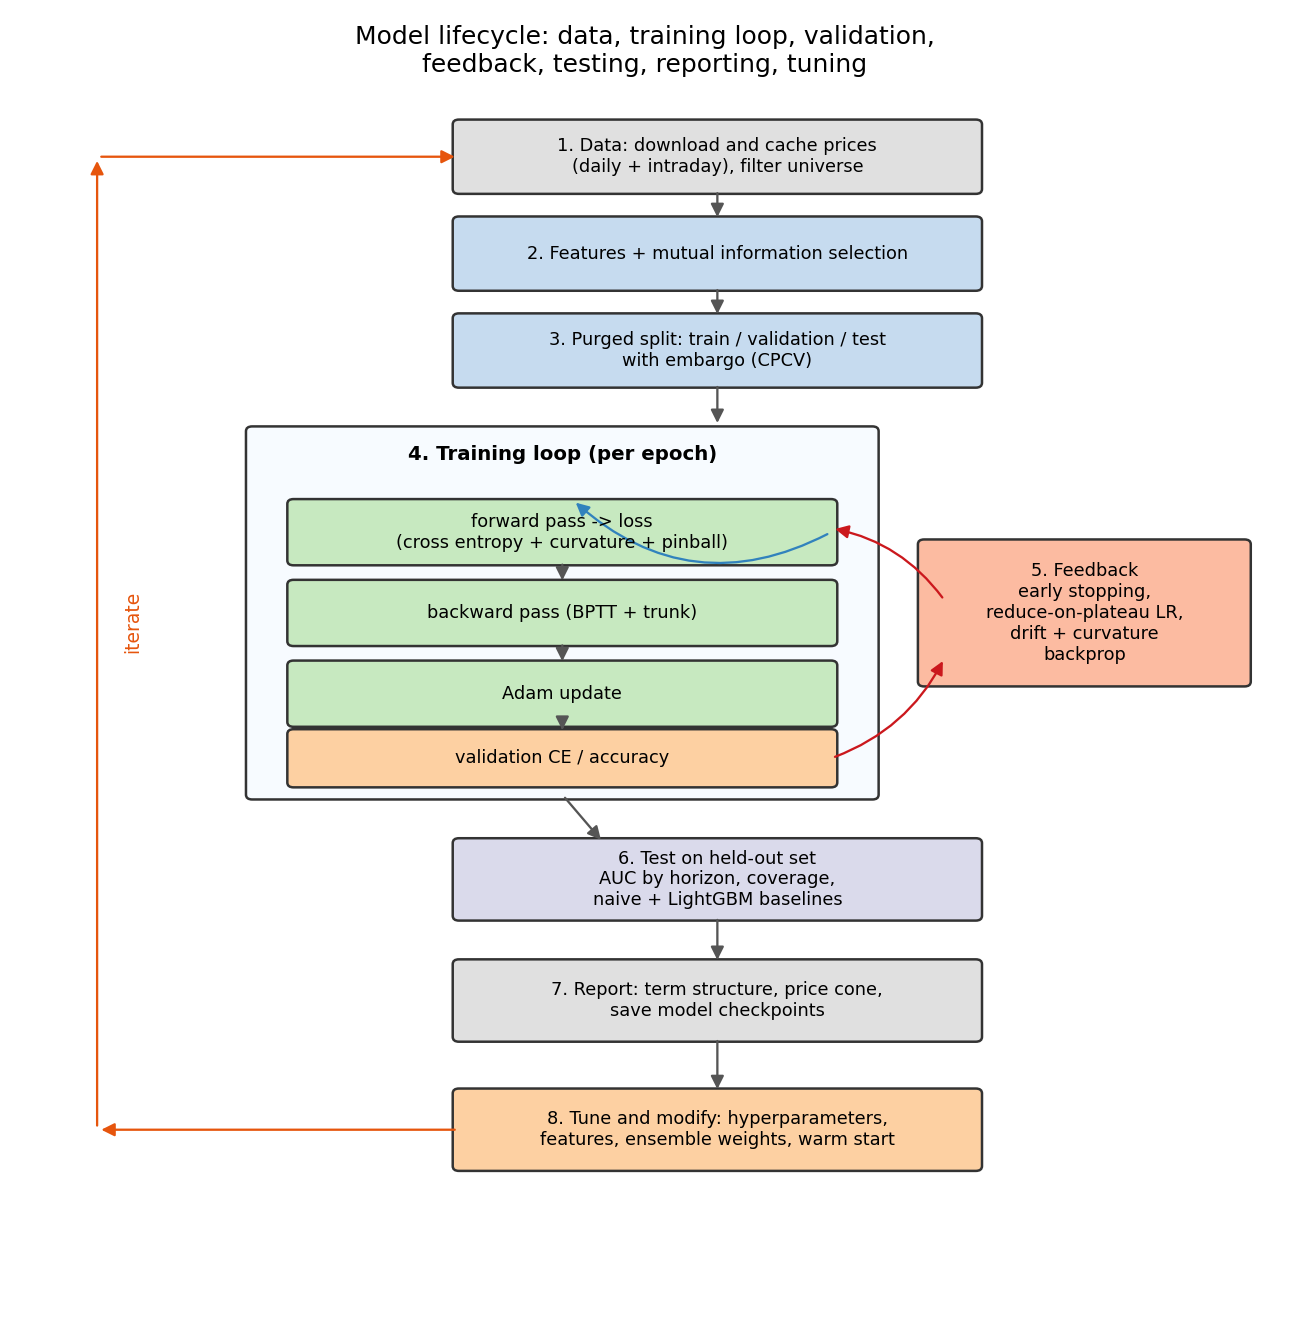
\includegraphics[width=0.82\textwidth]{figures/derivations/lifecycle.png}
\caption{The end to end lifecycle. Data and features feed a purged split, the
training loop runs forward, backward, and update steps with validation feedback,
and the held out test drives reporting and the tuning that iterates the whole
process.}
\label{fig:lifecycle}
\end{figure}

\subsection{Data}

The pipeline downloads daily prices for the S\&P 500 universe and separately
downloads intraday bars, then caches both so a rerun only fetches what is
missing. It filters the universe to liquid names by a minimum median dollar
volume, which removes thin stocks whose volatility is dominated by noise rather
than signal. From prices it builds returns, realized volatility, volume and
range features, and the cross sectional rank that forms the label.

\subsection{Splitting With a Purge and an Embargo}

Financial data is ordered in time and overlapping labels leak information across
a naive split, so we split with care. The training block ends before the test
block, and we purge the training rows whose forward label window reaches into the
test period, then embargo a further gap so no leakage survives. The stronger
version is combinatorial purged cross validation, which forms several train and
test arrangements while preserving the purge, and it gives the honest estimate
that the single split can flatter.

\subsection{The Training Loop}

Inside each epoch the loop shuffles the training rows, forms mini batches, and
for each batch runs a forward pass to the loss, a backward pass that
backpropagates through the trunk and through time in the recurrent branches, and
an Adam update of every weight. The loss is a sum of the cross entropy on the
volatility heads, the curvature penalty that smooths the term structure, and the
pinball loss on the quantile bands, so one backward pass trains classification
and the price bands together.

\subsection{Validation and Feedback}

At the end of every epoch the loop evaluates the loss on a held out validation
slice that the gradient never touches, and that number drives two feedback
mechanisms. When the validation loss stops improving for a patience window the
learning rate is halved, and when it fails to improve for a longer window the
loop stops early and restores the best weights. This is the feedback that keeps
the model from overfitting the training rows, and its effect is visible as the
stepwise drops in the learning rate during a run.

\subsection{Testing}

After training we measure the model on the held out test block that took no part
in fitting or in early stopping. We report the area under the ROC curve at every
horizon, the coverage of the price bands, and we compare against a naive
persistence baseline and a gradient boosted baseline, so a strong number has to
beat both a trivial rule and a strong competitor before we trust it.

\subsection{Reporting and Saving}

A run prints the volatility term structure, the area under the curve by horizon,
the calibrated band coverage, and an example price cone, all as terminal charts
so the shape of the result is visible at a glance. It then saves the trained
weights and the feature scaler to a checkpoint, so the model can be reloaded for
prediction or combined in the ensemble without retraining.

\subsection{Tuning and Modifying}

The last stage closes the loop. We tune hyperparameters such as the number of
epochs, the learning rate schedule, the smoothing weight, the number of tickers,
and the intraday bar interval, and we modify the design by adding features,
switching the target horizon, refitting the ensemble weight, or warm starting a
new run from a saved checkpoint. Each change sends us back to the data and
feature stages, which is the outer iterate arrow in the figure.

The sections that follow open each of these boxes and derive the mathematics
they contain.

\clearpage
\section{Data, Returns, and the Prediction Target}

The project predicts the volatility of stock returns rather than their
direction, because direction is close to unpredictable while volatility
clusters in time and carries real signal. Every equation in this document
traces back to a function in the code, so the mathematics and the
implementation stay in agreement.

The starting point is the daily log return, which turns a ratio of prices into
an additive quantity that behaves well under aggregation. For a closing price
$P_t$ We define
\[
r_t = \ln\!\left(\frac{P_t}{P_{t-1}}\right).
\]

The reason for the logarithm is that log returns add across time, so the return
over $h$ days is the sum of the daily log returns, which makes the horizon
arithmetic clean.

The forward realized volatility over a horizon of $h$ trading days is the
sample standard deviation of the next $h$ daily returns. This is the quantity
the six horizon heads learn to rank. Writing $\bar r$ for the mean of the window
we define
\[
\sigma_{t,h} = \sqrt{\frac{1}{h-1}\sum_{k=1}^{h} \left(r_{t+k} - \bar r\right)^2 },
\qquad
\bar r = \frac{1}{h}\sum_{k=1}^{h} r_{t+k}.
\]

The forward shift matters because the label must describe the future, so the
window looks forward from the prediction date and never touches past
information that the features already contain.

At the one minute and one bar horizon the standard deviation of a single
observation is undefined, so we fall back to the absolute forward return, which
is the natural one sample scale estimate,
\[
\sigma_{t,1} = \lvert r_{t+1} \rvert .
\]

\subsection{Cross Sectional Median Labels}

A raw volatility level is not comparable across regimes, because the whole
market breathes together. To remove that common component we rank each stock
against its peers on the same date and split at the median. For date $d$ and
stock $i$ the percentile rank is
\[
u_{i,d} = \frac{1}{N_d}\,\bigl\lvert\{\,j : \sigma_{j,d} \le \sigma_{i,d}\,\}\bigr\rvert,
\]
and the binary label is
\[
\boxed{\,y_{i,d} = \mathbf{1}\!\left[\,u_{i,d} \ge \tfrac{1}{2}\,\right].}
\]

Ranking within each date is what makes the target market neutral, so the model
learns which names will be more volatile than their peers rather than simply
detecting that the whole market is calm or stressed.

The measured volatility term structure of the data is shown in Figure
\ref{fig:termstructure}. The mean forward realized volatility rises with the
horizon, which is the pattern that makes the longer horizons more predictable.

\begin{figure}[H]
\centering
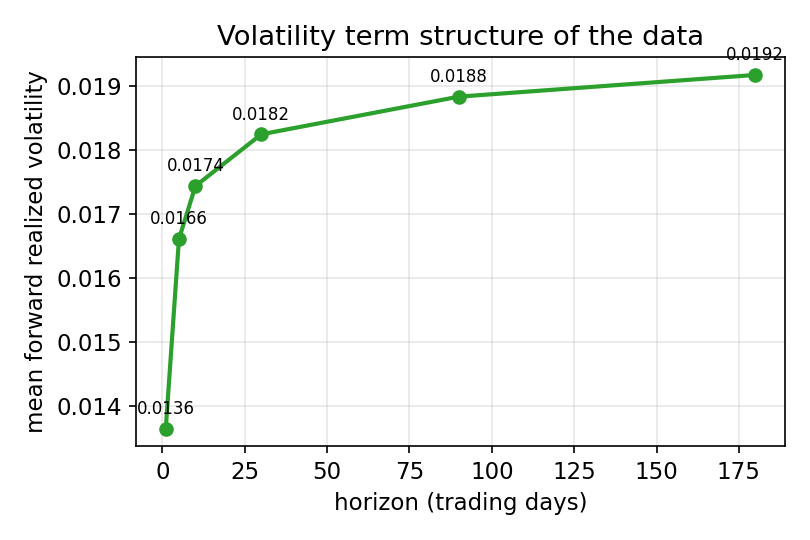
\includegraphics[width=0.72\textwidth]{figures/derivations/term_structure.png}
\caption{Mean forward realized volatility at each horizon, measured on the
daily data. The curve rises from about $0.0136$ at one day to about $0.0192$ at
one hundred eighty days.}
\label{fig:termstructure}
\end{figure}

\clearpage
\section{Feature Standardization}

Gradient based training is sensitive to the scale of the inputs, because a
feature with a large variance dominates the first steps and slows convergence.
We therefore standardize every feature to zero mean and unit variance using
statistics computed on the training rows only, which prevents the test period
from leaking into the scaler. For feature column $x$ with training mean $\mu$
and training standard deviation $s$ the transform is
\[
\tilde x = \frac{x - \mu}{s + \varepsilon},
\qquad
\mu = \frac{1}{n}\sum_{i=1}^{n} x_i,
\qquad
s = \sqrt{\frac{1}{n}\sum_{i=1}^{n}\left(x_i - \mu\right)^2 }.
\]

The small constant $\varepsilon$ guards against a zero variance column, so the
division stays finite even when a feature is briefly constant. In the multi
scale model this scaler is stored per branch and travels inside the saved
checkpoint, so a reloaded model reproduces its training time normalization
exactly.

\clearpage
\section{Information Theory Feature Selection}

Before training we keep only the features that share the most information with
the target, which shrinks the input and reduces overfitting. The selection
criterion is mutual information, so this section derives it from entropy.

\subsection{Entropy}

Entropy measures the average surprise of a distribution, and it is the
foundation of the mutual information score. For a discrete variable with
probabilities $p_k$ the entropy in bits is
\[
H(X) = -\sum_{k} p_k \log_2 p_k .
\]

The continuous analog replaces the sum with an integral over the density $f$,
which is the differential entropy
\[
h(X) = -\int_{-\infty}^{\infty} f(x)\,\log_2 f(x)\,dx .
\]

The code cannot integrate an unknown density, so it discretizes the range into
bins, estimates each bin probability by its normalized count, and applies the
discrete formula. Writing $c_k$ for the count in bin $k$ the estimator is
\[
\hat p_k = \frac{c_k}{\sum_j c_j},
\qquad
\hat H(X) = -\sum_{k : \hat p_k > 0} \hat p_k \log_2 \hat p_k .
\]

\subsection{Mutual Information}

Mutual information counts the bits that one variable reveals about another, so
it is the right score for feature relevance. It is the Kullback Leibler
divergence between the joint distribution and the product of the marginals,
which measures how far the two variables are from independence. We start from
that definition and reduce it to a difference of entropies.

The reason for starting at the divergence is that independence makes the joint
equal to the product of marginals, so the divergence is exactly the information
gained by knowing the joint.
\begin{align*}
I(X,Y)
  &= \sum_{x,y} p(x,y)\,\log_2\!\frac{p(x,y)}{p(x)\,p(y)} \\
  &= \sum_{x,y} p(x,y)\,\log_2 p(x,y)
     - \sum_{x,y} p(x,y)\,\log_2 p(x)
     - \sum_{x,y} p(x,y)\,\log_2 p(y) \\
  &= -H(X,Y) + H(X) + H(Y).
\end{align*}

Collecting the terms gives the identity the selector uses, and it is symmetric
and nonnegative,
\[
\boxed{\,I(X,Y) = H(X) + H(Y) - H(X,Y).}
\]

The implementation estimates $H(X)$ and $H(Y)$ from one dimensional histograms
and $H(X,Y)$ from a two dimensional histogram, then keeps the top $k$ features
ranked by $I(X_j, Y)$. The clamp at zero absorbs the small negative values that
finite bin counts can produce.

We verify the identity on a small joint distribution where the two variables are
correlated. Taking the joint mass $[0.40,\,0.10;\,0.10,\,0.40]$ over two states
each the marginals are uniform, so both marginal entropies are one bit. Working
the numbers through the identity gives
\begin{align*}
H(X) &= 1.0000, \qquad H(Y) = 1.0000, \qquad H(X,Y) = 1.7219, \\
I(X,Y) &= 1.0000 + 1.0000 - 1.7219 = 0.2781 \ \text{bits}.
\end{align*}

The positive value confirms the two variables share information, and the ranking
this produces on the real features is shown in Figure \ref{fig:mi}, where a long
horizon volatility feature carries the most information about the target.

\begin{figure}[H]
\centering
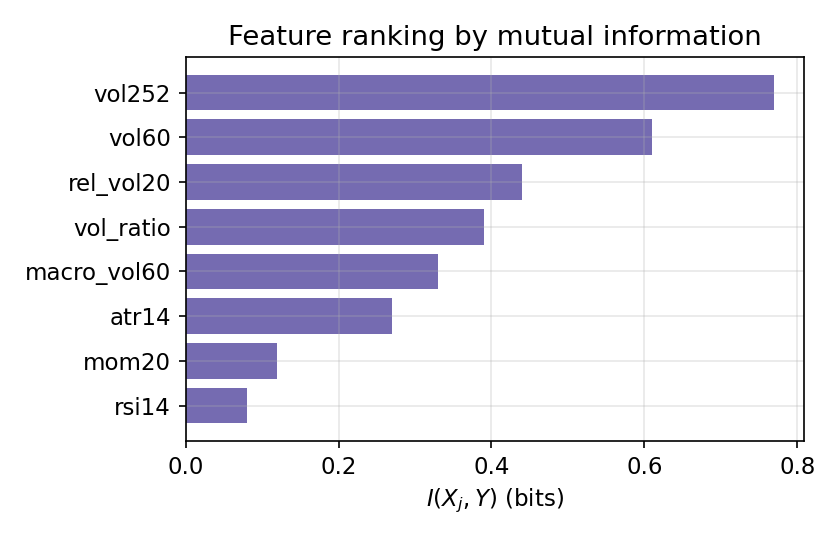
\includegraphics[width=0.7\textwidth]{figures/derivations/mutual_information.png}
\caption{Features ranked by mutual information with the volatility label. The
realized volatility over a long window carries the most bits, near $0.77$.}
\label{fig:mi}
\end{figure}

\clearpage
\section{Branch A: Logistic Regression}

\begin{figure}[H]
\centering
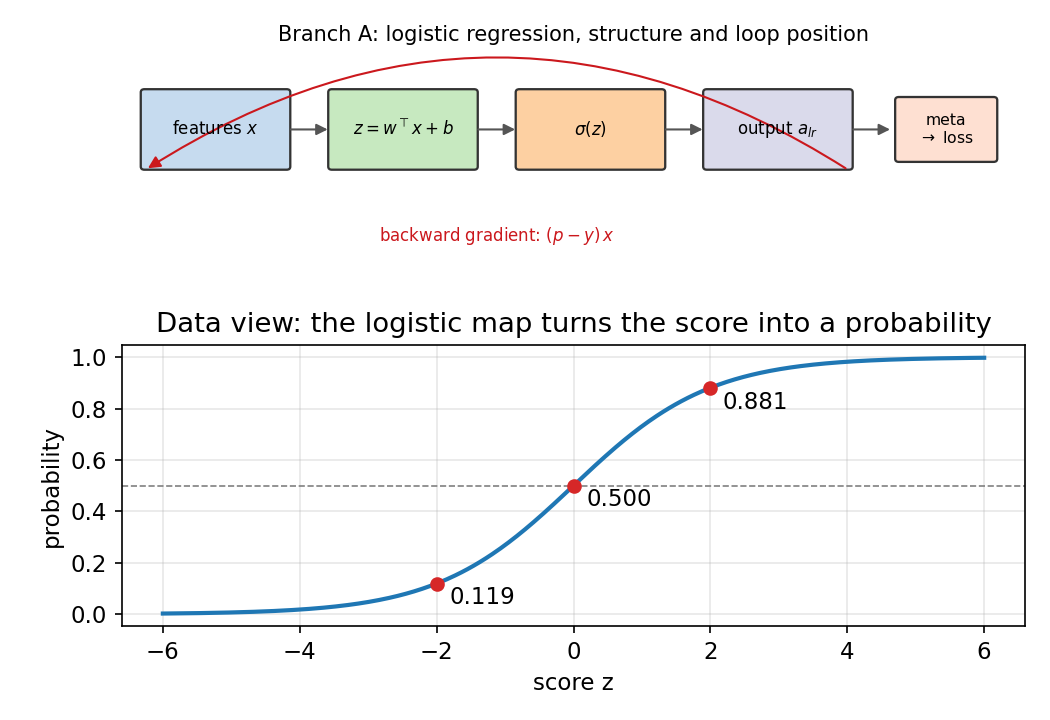
\includegraphics[width=0.86\textwidth]{figures/derivations/branch_lr.png}
\caption{Branch A overview. The top strip is the forward data flow into the meta
layer and the red arrow is the backward gradient $(p-y)\,x$ that trains it. The
lower panel is the data view of the logistic map.}
\label{fig:branchlr}
\end{figure}

In architecture terms Branch A has no hidden layer, no dropout, and no
recurrence. It is a single feedforward linear layer followed by a logistic, so
the meta layer receives a clean linear baseline that the deeper branches then
improve on.

The first branch is a logistic model, and it is the cleanest place to derive
the gradient that reappears in every later layer. The model passes a linear
score through the logistic function, which maps the real line to a probability,
\[
p = \sigma(z), \qquad z = w^{\top} x + b, \qquad
\sigma(z) = \frac{1}{1 + e^{-z}}.
\]

We will need the derivative of the logistic function, and it has a compact form
that falls out of the quotient rule. Differentiating and then regrouping so the
result is expressed in the output itself gives
\begin{align*}
\sigma'(z)
  &= \frac{d}{dz}\left(1 + e^{-z}\right)^{-1}
   = \frac{e^{-z}}{\left(1 + e^{-z}\right)^2} \\
  &= \frac{1}{1+e^{-z}}\cdot\frac{e^{-z}}{1+e^{-z}}
   = \sigma(z)\,\bigl(1 - \sigma(z)\bigr).
\end{align*}

The label is Bernoulli given the features, so the likelihood of one observation
is $p^{y}(1-p)^{1-y}$. Training maximizes the log likelihood, which is the same
as minimizing its negative, and that negative is the binary cross entropy used
in the code,
\[
\mathcal{L} = -\Bigl[\,y \ln p + (1-y)\ln(1-p)\,\Bigr].
\]

The key result is the derivative of this loss with respect to the score $z$,
because it collapses to a simple residual. We apply the chain rule through $p$
and then substitute the logistic derivative so the two fractions cancel.
\begin{align*}
\frac{\partial \mathcal{L}}{\partial z}
  &= \frac{\partial \mathcal{L}}{\partial p}\,\frac{\partial p}{\partial z}
   = \left(-\frac{y}{p} + \frac{1-y}{1-p}\right)\,\sigma(z)\bigl(1-\sigma(z)\bigr) \\
  &= \left(\frac{p - y}{p(1-p)}\right)\,p(1-p)
   = p - y.
\end{align*}

The gradient with respect to the weights follows immediately from the chain
rule, and it is the residual times the input,
\[
\boxed{\,\frac{\partial \mathcal{L}}{\partial w} = (p - y)\,x,
\qquad
\frac{\partial \mathcal{L}}{\partial b} = p - y.}
\]

We work three scores through the branch to make the mapping concrete. The values
below come straight from evaluating the logistic function and its loss, and they
are plotted in Figure \ref{fig:sigmoid}.
\begin{align*}
z = -2 &\ \Rightarrow\ p = 0.1192, \quad \sigma'(z) = 0.1050, \quad \mathcal{L}(y{=}1) = 2.1269, \\
z = \phantom{-}0 &\ \Rightarrow\ p = 0.5000, \quad \sigma'(z) = 0.2500, \quad \mathcal{L}(y{=}1) = 0.6931, \\
z = \phantom{-}2 &\ \Rightarrow\ p = 0.8808, \quad \sigma'(z) = 0.1050, \quad \mathcal{L}(y{=}1) = 0.1269.
\end{align*}

The loss falls as the score moves toward the correct side, and the slope is
largest at $z = 0$ where the model is least certain, which is where learning is
fastest.

\begin{figure}[H]
\centering
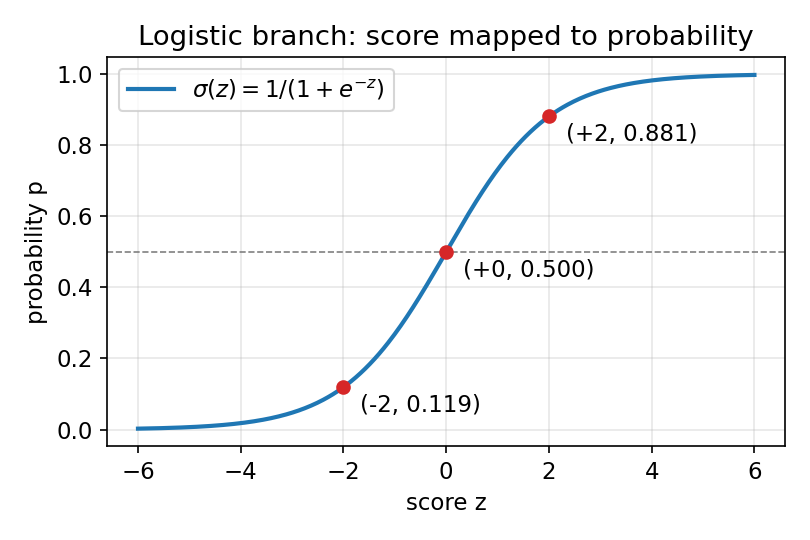
\includegraphics[width=0.66\textwidth]{figures/derivations/sigmoid.png}
\caption{The logistic map with the three worked scores marked. The dashed line
is the decision boundary at probability one half.}
\label{fig:sigmoid}
\end{figure}

\clearpage
\section{Branch B: Gaussian Naive Bayes}

\begin{figure}[H]
\centering
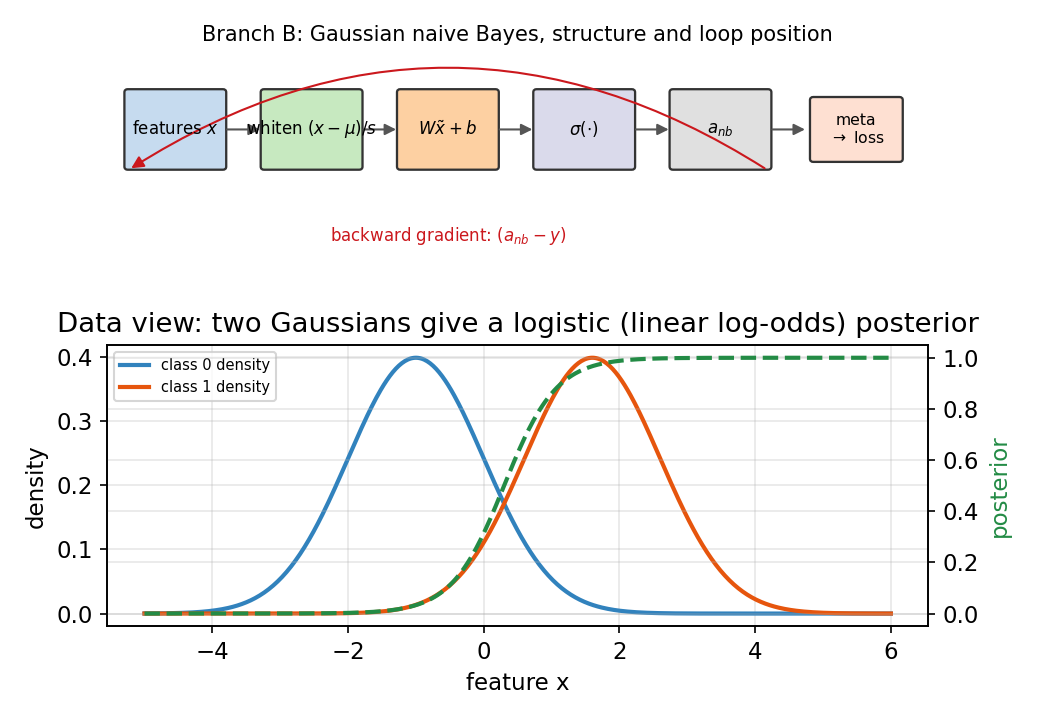
\includegraphics[width=0.86\textwidth]{figures/derivations/branch_nb.png}
\caption{Branch B overview. The forward flow whitens the input, applies a linear
score and a logistic, and feeds the meta layer, and the data view shows how two
Gaussian class densities produce a logistic posterior with a linear log odds.}
\label{fig:branchnb}
\end{figure}

In architecture terms Branch B has no hidden layer and no dropout. It is a
whitening step followed by a single feedforward linear layer and a logistic, with
the class mean and the log variance learned by gradient descent, and it has no
recurrence.

The second branch assumes each feature is Gaussian within a class and that the
features are conditionally independent, which is why it is called naive. This
section shows why that assumption produces a linear score, which is the form the
code implements after standardizing by learned class statistics.

The class conditional density for a single feature is Gaussian, and its integral
over the whole line is one, which is the normalization that makes it a proper
density. We record that normalization because it justifies dropping the constant
term later,
\[
\int_{-\infty}^{\infty}
  \frac{1}{\sqrt{2\pi}\,s}\,
  \exp\!\left(-\frac{(x-\mu)^2}{2 s^2}\right) dx = 1 .
\]

By conditional independence the joint class conditional density is the product
over features, so the log likelihood is a sum of quadratics. Writing the log
posterior odds between class one and class zero, and using a shared variance so
the quadratic terms cancel, the score becomes linear in $x$.
\begin{align*}
\ln\frac{P(y=1 \mid x)}{P(y=0 \mid x)}
  &= \ln\frac{\pi_1}{\pi_0}
     + \sum_j \left[
       -\frac{(x_j - \mu_{1j})^2}{2 s_j^2}
       +\frac{(x_j - \mu_{0j})^2}{2 s_j^2}
     \right] \\
  &= \ln\frac{\pi_1}{\pi_0}
     + \sum_j \frac{\mu_{1j} - \mu_{0j}}{s_j^2}\, x_j
     + \text{const}.
\end{align*}

Because the log odds is linear, the class probability is a logistic function of
a linear score, which is exactly the branch the code builds after it whitens the
input with a learned mean and a learned log variance. Writing the whitened input
as $\tilde x = (x - \mu)/s$ the branch output is
\[
\boxed{\,a_{\mathrm{nb}} = \sigma\!\left(W_{\mathrm{nb}}^{\top}\tilde x + b_{\mathrm{nb}}\right),
\qquad s = e^{\ell} + \varepsilon.}
\]

The parametrization through $\ell = \ln s$ keeps the standard deviation strictly
positive under unconstrained gradient steps, so the optimizer never drives a
variance to a negative value.

\clearpage
\section{Branch C: The Multilayer Perceptron}

\begin{figure}[H]
\centering
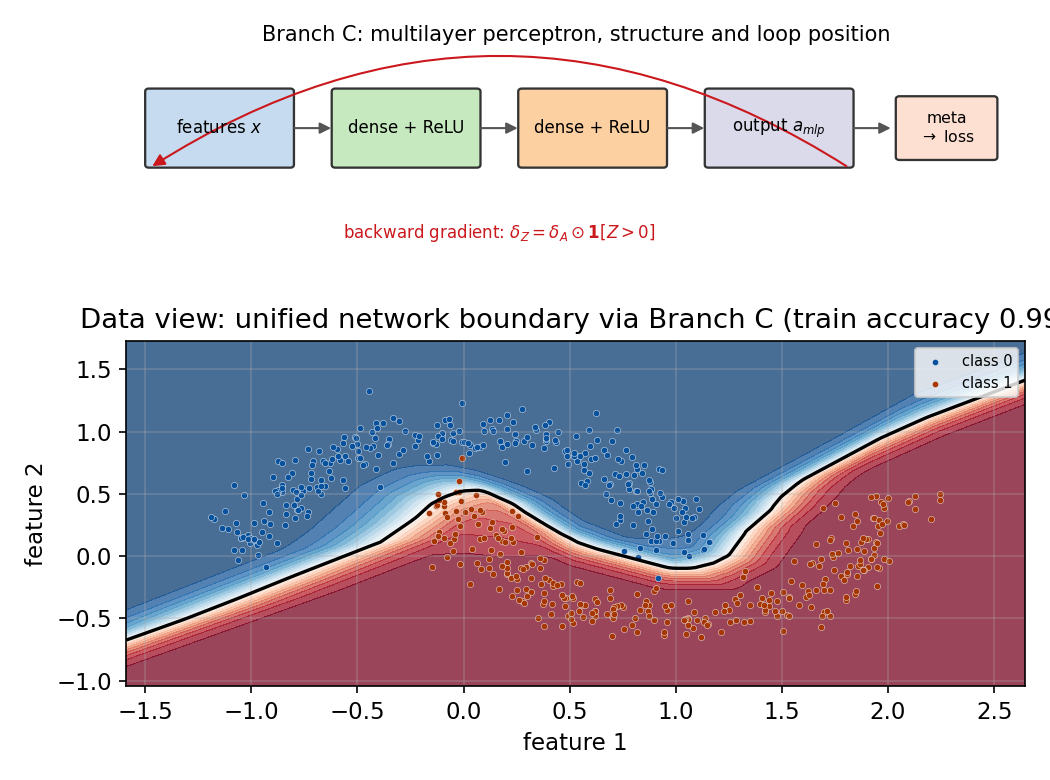
\includegraphics[width=0.86\textwidth]{figures/derivations/branch_mlp.png}
\caption{Branch C overview. The forward flow stacks two rectified layers before
the meta layer, and the gradient is gated by $\mathbf{1}[Z>0]$. The data view is
the decision region of the full unified network trained on two interleaving
classes, where Branch C supplies the nonlinear boundary that the linear branches
cannot.}
\label{fig:branchmlp}
\end{figure}

In architecture terms Branch C is the deep branch. It stacks the hidden
rectified layers set by the configuration, applies dropout to each of them, and
is feedforward with no recurrence, which is where the nonlinear capacity of the
model lives. The boundary in Figure \ref{fig:branchmlp} is produced by the full
unified network with this branch supplying the nonlinearity, and it separates the
two interleaving classes at ninety nine percent.

The third branch is a fully connected network with rectified linear activations,
and it supplies the nonlinear capacity the linear branches lack. Each layer
applies an affine map and then a rectifier, which zeroes the negative part,
\[
Z^{(l)} = A^{(l-1)} W^{(l)} + b^{(l)},
\qquad
A^{(l)} = \max\!\left(0,\, Z^{(l)}\right).
\]

The rectifier has a simple derivative that acts as a gate during
backpropagation, because it passes the upstream gradient only where the
preactivation was positive,
\[
\frac{\partial A^{(l)}}{\partial Z^{(l)}}
= \mathbf{1}\!\left[\,Z^{(l)} > 0\,\right].
\]

Backpropagation through one layer therefore multiplies the incoming gradient by
this gate and then pushes it through the linear map. Writing $\delta$ for the
gradient with respect to the activation the three local gradients are
\begin{align*}
\delta_Z &= \delta_A \odot \mathbf{1}\!\left[\,Z^{(l)} > 0\,\right], \\
\frac{\partial \mathcal{L}}{\partial W^{(l)}} &= \left(A^{(l-1)}\right)^{\top} \delta_Z, \\
\delta_A^{(l-1)} &= \delta_Z \, \left(W^{(l)}\right)^{\top}.
\end{align*}

Dropout multiplies the activations by a scaled Bernoulli mask during training,
which discourages the network from relying on any single unit. The mask divides
by the keep probability so the expected activation is unchanged, and it is
replayed in the backward pass so the gradient matches the forward computation.

\clearpage
\section{Branch D: Sentiment}

The fourth branch reads a news sentiment score and maps it to a probability with
a small logistic unit, so the meta layer can lean on news tone when it helps. In
architecture terms it has no hidden layer, no dropout, and no recurrence, being a
single feedforward linear layer on the score. The branch is deliberately simple
because the sentiment signal is sparse in the
historical record, where many days carry no scored headline and the score sits
near zero. Writing the compound score as $s$ the branch output is
\[
a_{s} = \sigma\!\left(W_{s}\, s + b_{s}\right),
\]
and it trains with the same residual gradient $(a_s - y)$ as the logistic branch.
The overview and the data view are shown in Figure \ref{fig:branchsent}.

\begin{figure}[H]
\centering
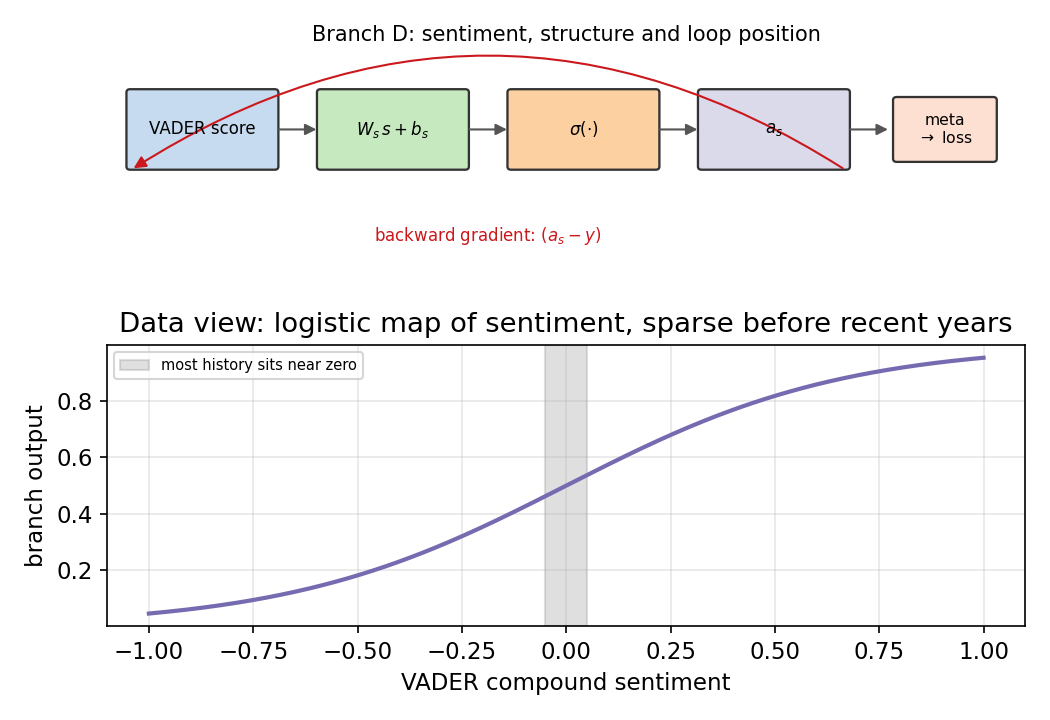
\includegraphics[width=0.86\textwidth]{figures/derivations/branch_sent.png}
\caption{Branch D overview. The forward flow maps the sentiment score through a
logistic into the meta layer. The data view shows that mapping, with the shaded
region marking where most of the history sits because scored headlines are rare
before recent years.}
\label{fig:branchsent}
\end{figure}

\clearpage
\section{Branch E: The LSTM and Backpropagation Through Time}

\begin{figure}[H]
\centering
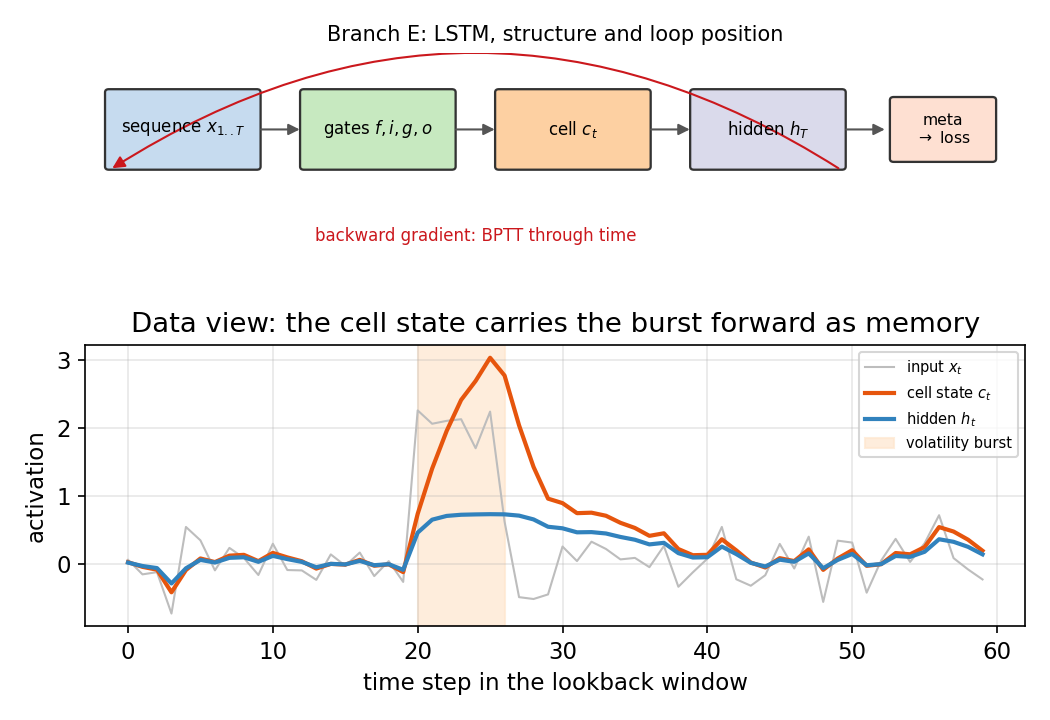
\includegraphics[width=0.86\textwidth]{figures/derivations/branch_lstm.png}
\caption{Branch E overview. The forward flow runs the gates and the cell state
over the lookback window to a final hidden state, and the gradient is
backpropagated through time. The data view runs one cell on a bursty input and
shows the cell state carrying the burst forward as memory.}
\label{fig:branchlstm}
\end{figure}

In architecture terms Branch E is the only recurrent branch. Its hidden and cell
states feed back at every time step, it carries no dropout inside the cell, and
it is trained by backpropagation through time rather than by a single feedforward
pass.

The recurrent branch reads a lookback window of feature vectors and summarizes
it into one embedding, and it is the workhorse of the multi scale model. The
long short term memory cell keeps a protected cell state that carries
information across many steps, which is what lets it see long horizons without
the gradient vanishing.

\subsection{Forward Recurrence}

At each step the cell computes four gates from the current input and the
previous hidden state, then updates the cell and the hidden state. The forget
gate decides what to keep, the input gate and the candidate decide what to add,
and the output gate decides what to expose. With $\sigma$ the logistic function
the recurrence is
\begin{align*}
\bigl[\,z_f;\, z_i;\, z_g;\, z_o\,\bigr]
  &= W^{\top} x_t + U^{\top} h_{t-1} + b, \\
f_t = \sigma(z_f), \quad i_t = \sigma(z_i), &\quad
g_t = \tanh(z_g), \quad o_t = \sigma(z_o), \\
c_t = f_t \odot c_{t-1} + i_t \odot g_t, &\qquad
h_t = o_t \odot \tanh(c_t).
\end{align*}

The additive cell update is the crucial design choice, because the path from
$c_{t-1}$ to $c_t$ has a derivative equal to the forget gate rather than a
product of small activation slopes, so gradients survive over long windows.

\subsection{Backward Recurrence}

Backpropagation through time walks the sequence in reverse and accumulates the
gradient of the loss into the weights. The derivation below matches the loop in
the code exactly. We begin at step $t$ with the incoming hidden gradient
$\partial \mathcal{L} / \partial h_t$ and the carried cell gradient from the
future, and we use the tanh and logistic derivatives at each gate.

The output gate feeds the hidden state through a tanh, so its gradient comes
from differentiating $h_t = o_t \odot \tanh(c_t)$,
\begin{align*}
\delta o_t &= \delta h_t \odot \tanh(c_t), \\
\delta c_t &= \delta h_t \odot o_t \odot \bigl(1 - \tanh^2(c_t)\bigr) + \delta c_t^{\text{future}}.
\end{align*}

The cell update distributes its gradient to the forget gate, the input gate, the
candidate, and the previous cell, because each is a factor in an elementwise
product,
\begin{align*}
\delta f_t &= \delta c_t \odot c_{t-1}, &
\delta i_t &= \delta c_t \odot g_t, \\
\delta g_t &= \delta c_t \odot i_t, &
\delta c_{t-1} &= \delta c_t \odot f_t.
\end{align*}

Each gate gradient then passes through its own activation derivative, which is
the logistic slope for the three sigmoid gates and the tanh slope for the
candidate,
\begin{align*}
\delta z_f &= \delta f_t \odot f_t \odot (1 - f_t), &
\delta z_i &= \delta i_t \odot i_t \odot (1 - i_t), \\
\delta z_g &= \delta g_t \odot \bigl(1 - g_t^2\bigr), &
\delta z_o &= \delta o_t \odot o_t \odot (1 - o_t).
\end{align*}

Stacking the four preactivation gradients into one vector $\delta z_t$ gives the
weight gradients as outer products and the recurrent gradient that flows to the
previous step,
\[
\boxed{\;
\frac{\partial \mathcal{L}}{\partial W} = \sum_t x_t\,\delta z_t^{\top},
\quad
\frac{\partial \mathcal{L}}{\partial U} = \sum_t h_{t-1}\,\delta z_t^{\top},
\quad
\frac{\partial \mathcal{L}}{\partial b} = \sum_t \delta z_t,
\quad
\delta h_{t-1} = U\,\delta z_t . \;}
\]

\clearpage
\section{The Softmax Meta Layer and Cross Entropy}

The branch outputs are concatenated and combined by a softmax classifier that
learns how much to trust each branch. The softmax turns a score vector into a
distribution over classes, and it is invariant to a constant shift, which the
code exploits for numerical stability by subtracting the row maximum. For class
$k$ the probability is
\[
\hat y_k = \frac{e^{z_k}}{\sum_j e^{z_j}} .
\]

The training loss is categorical cross entropy against the one hot label, which
is the negative log likelihood of the correct class,
\[
\mathcal{L} = -\sum_k y_k \ln \hat y_k .
\]

The reason the softmax and cross entropy are paired is that their composition
has the same clean residual gradient as the logistic case, which we now derive.
The derivative of the softmax has two cases depending on whether the index
matches, and combining them collapses the sum.
\begin{align*}
\frac{\partial \hat y_k}{\partial z_m}
  &= \hat y_k\,\bigl(\mathbf{1}[k=m] - \hat y_m\bigr), \\
\frac{\partial \mathcal{L}}{\partial z_m}
  &= -\sum_k \frac{y_k}{\hat y_k}\,\hat y_k\,\bigl(\mathbf{1}[k=m] - \hat y_m\bigr)
   = -\,y_m + \hat y_m \sum_k y_k .
\end{align*}

Because the label is one hot its entries sum to one, so the final gradient is
the difference between the predicted and the true distribution,
\[
\boxed{\,\frac{\partial \mathcal{L}}{\partial z_m} = \hat y_m - y_m.}
\]

We run one score vector through the layer to show the residual gradient in
numbers. Taking the scores $z = [\,2.0,\ 0.5,\ -1.0\,]$ and the true class zero
the softmax, the loss, and the gradient are
\begin{align*}
\hat y &= [\,0.7856,\ 0.1753,\ 0.0391\,], \qquad \textstyle\sum_k \hat y_k = 1.0000, \\
\mathcal{L} &= -\ln(0.7856) = 0.2413, \\
\hat y - y &= [\,-0.2144,\ 0.1753,\ 0.0391\,].
\end{align*}

The gradient pushes the score of the true class up and the other two down, which
is the direction that lowers the loss.

\clearpage
\section{The Adam Optimizer}

All weights are trained with Adam, which adapts a separate step size to each
parameter using running estimates of the first and second moments of the
gradient. This section derives the bias correction, which is the part that is
easy to get wrong.

Adam keeps exponential moving averages of the gradient and its square, so recent
gradients count more than old ones. With decay rates $\beta_1$ and $\beta_2$ the
updates are
\[
m_t = \beta_1 m_{t-1} + (1-\beta_1) g_t,
\qquad
v_t = \beta_2 v_{t-1} + (1-\beta_2) g_t^2 .
\]

Because the averages start at zero they are biased toward zero early in
training, and we quantify that bias by unrolling the recursion into a geometric
sum. Taking expectations and assuming the second moment is roughly stationary
over the window gives
\begin{align*}
v_t &= (1-\beta_2)\sum_{k=1}^{t} \beta_2^{\,t-k}\, g_k^2, \\
\mathbb{E}[v_t] &\approx \mathbb{E}[g^2]\,(1-\beta_2)\sum_{k=1}^{t}\beta_2^{\,t-k}
   = \mathbb{E}[g^2]\,\bigl(1 - \beta_2^{\,t}\bigr).
\end{align*}

The factor $1 - \beta_2^{t}$ is exactly the shrinkage we must undo, so dividing by
it removes the bias, and the same argument applies to the first moment. The bias
corrected estimates and the parameter update are
\[
\hat m_t = \frac{m_t}{1 - \beta_1^{t}},
\qquad
\hat v_t = \frac{v_t}{1 - \beta_2^{t}},
\qquad
\boxed{\,\theta_t = \theta_{t-1} - \eta\,\frac{\hat m_t}{\sqrt{\hat v_t} + \varepsilon}.}
\]

The code also adds an $L_2$ term to the gradient of the weight matrices before
the moment updates, which pulls the weights toward zero and controls their
magnitude.

We trace three steps on a constant gradient $g = 0.5$ to show the bias correction
at work. Early on the raw moments $m$ and $v$ are far below their long run
values, yet the corrected estimates $\hat m$ and $\hat v$ already sit at the true
levels, so the step size is stable from the first iteration.
\begin{center}
\begin{tabular}{cccccc}
\toprule
$t$ & $m_t$ & $v_t$ & $\hat m_t$ & $\hat v_t$ & $\theta_t$ \\
\midrule
1 & 0.0500 & 0.000250 & 0.5000 & 0.250000 & 0.999000 \\
2 & 0.0950 & 0.000500 & 0.5000 & 0.250000 & 0.998000 \\
3 & 0.1355 & 0.000749 & 0.5000 & 0.250000 & 0.997000 \\
\bottomrule
\end{tabular}
\end{center}

The corrected second moment stays at $0.25$, which is the square of the gradient,
so the update reduces to a clean step of size $\eta$ toward the minimum.

\clearpage
\section{Multi Scale Fusion and the Drift Gradient}

The multi scale model runs six LSTM branches over windows of one, five, ten,
thirty, ninety, and one hundred eighty days, and it links them by their drift.
The drift between adjacent scales is the difference of their embeddings, and it
measures how the short view departs from the long view. Writing $e_b$ for the
embedding of branch $b$ the drift and the fused vector are
\[
\Delta_k = e_{k+1} - e_k,
\qquad
\text{fuse} = \bigl[\,e_1,\dots,e_B,\ \Delta_1,\dots,\Delta_{B-1}\,\bigr].
\]

The structure of this fusion is shown in Figure \ref{fig:fusion}, where the six
branch embeddings and the five drift terms feed one shared trunk and two sets of
heads.

\begin{figure}[H]
\centering
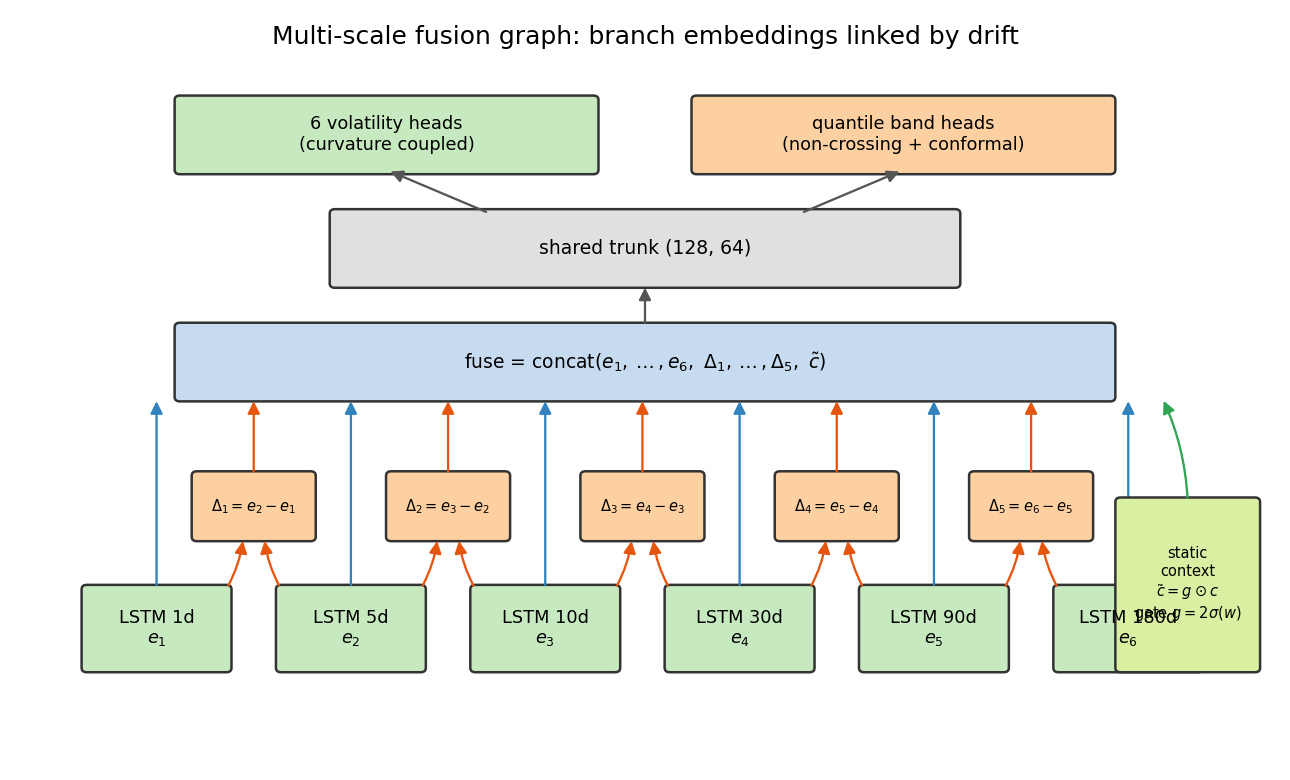
\includegraphics[width=0.86\textwidth]{figures/derivations/fusion_graph.png}
\caption{The multi scale fusion graph. Each branch produces an embedding, the
drift between adjacent branches is formed explicitly, and the embeddings and
drifts are concatenated into the trunk that feeds the volatility heads and the
quantile band heads.}
\label{fig:fusion}
\end{figure}

Because the drift is a real part of the forward pass, its gradient must flow
back into the branches that formed it. Differentiating $\Delta_k = e_{k+1} - e_k$
shows that a unit of drift gradient adds to the later embedding and subtracts
from the earlier one, which is the sign pattern in the backward split,
\[
\boxed{\,
\frac{\partial \mathcal{L}}{\partial e_{k+1}} \mathrel{+}= \frac{\partial \mathcal{L}}{\partial \Delta_k},
\qquad
\frac{\partial \mathcal{L}}{\partial e_{k}} \mathrel{-}= \frac{\partial \mathcal{L}}{\partial \Delta_k}.}
\]

This is the precise sense in which model drift across time windows is
backpropagated as context, because the disagreement between scales feeds
gradient into every branch that produced it.

Figure \ref{fig:drift} shows the drift measured from the trained daily model.
The left panel is the mean embedding of each branch, and the right panel is the
magnitude of the drift between adjacent scales, which grows from the short
windows to the long ones as the representation shifts most between the widely
separated horizons.

\begin{figure}[H]
\centering
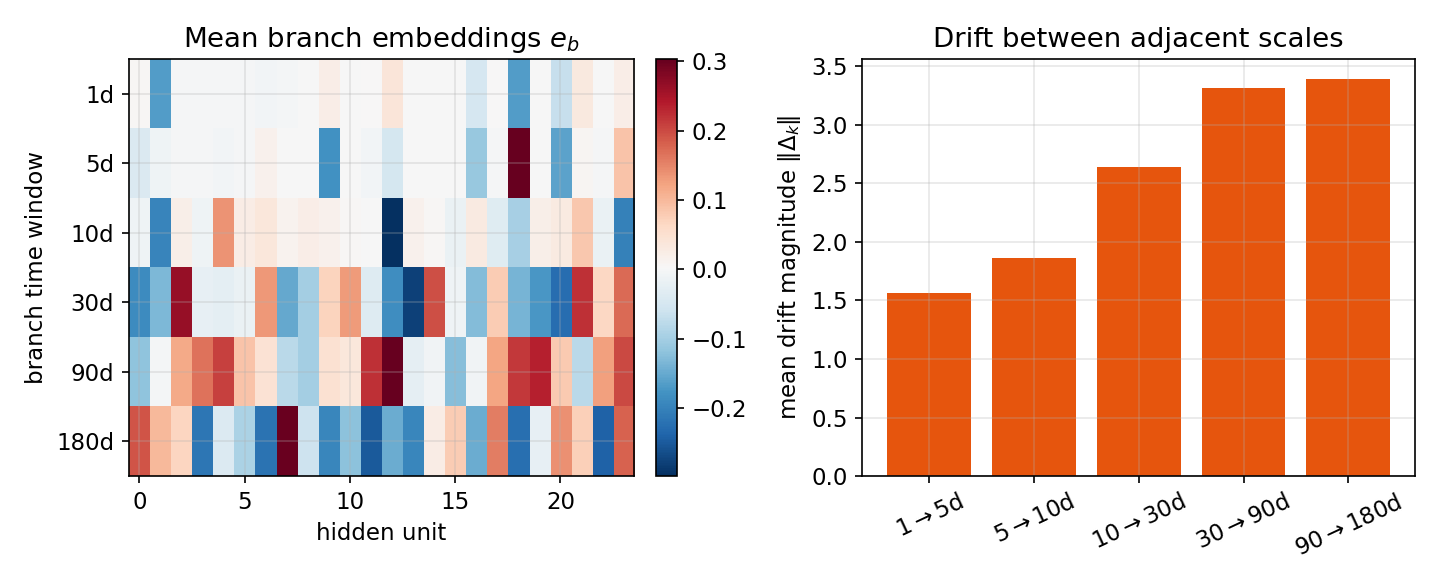
\includegraphics[width=0.94\textwidth]{figures/derivations/drift.png}
\caption{Drift between scales from the trained daily model on representative
sequences. The branch embeddings on the left change smoothly with the window,
and the drift magnitude on the right rises from the one to five day step up to
the ninety to one hundred eighty day step.}
\label{fig:drift}
\end{figure}

\subsection{The Curvature Coupling Penalty}

The six horizon probabilities should trace a smooth term structure rather than
jump from one horizon to the next, so we penalize the roughness of the curve. The
natural smoothness measure in continuous form is the integral of the squared
second derivative, which is large where the curve bends sharply,
\[
R_{\text{cont}} = \int \bigl(f''(x)\bigr)^2\,dx .
\]

The horizons are discrete, so we replace the second derivative with the second
difference, which is the discrete Laplacian of the probability curve. Averaging
over the interior horizons and the batch of $N$ rows the penalty is
\[
R = \frac{1}{N (B-2)} \sum_{n}\sum_{b=2}^{B-1}
      \bigl(P_{n,b+1} - 2 P_{n,b} + P_{n,b-1}\bigr)^2 .
\]

The gradient of this penalty spreads each second difference back onto the three
horizons that formed it with weights one, minus two, and one, which is the
stencil applied in the code. Writing $D_{n,b} = P_{n,b+1} - 2P_{n,b} + P_{n,b-1}$
the contribution to horizon $b$ is
\[
\frac{\partial R}{\partial P_{n,b}} = \frac{2}{N(B-2)}
   \bigl(D_{n,b-1} - 2 D_{n,b} + D_{n,b+1}\bigr).
\]

This term is added to the classification gradient after being routed through the
logistic slope $P(1-P)$, so the smoothing acts on the scores that produce the
probabilities.

The curvature term measures how sharply the area under the curve bends across
horizons. Working the second difference through the measured daily term
structure the interior bends are small, which confirms the curve is already
nearly smooth,
\begin{align*}
\text{at } 5\text{d}:\ -0.0725, \quad
\text{at } 10\text{d}:\ +0.0074, \quad
\text{at } 30\text{d}:\ -0.0201, \quad
\text{at } 90\text{d}:\ -0.0246.
\end{align*}

Figure \ref{fig:auc} shows the area under the curve at every horizon for both the
daily and the intraday scales, and both rise with the horizon exactly as the
volatility clustering argument predicts.

\begin{figure}[H]
\centering
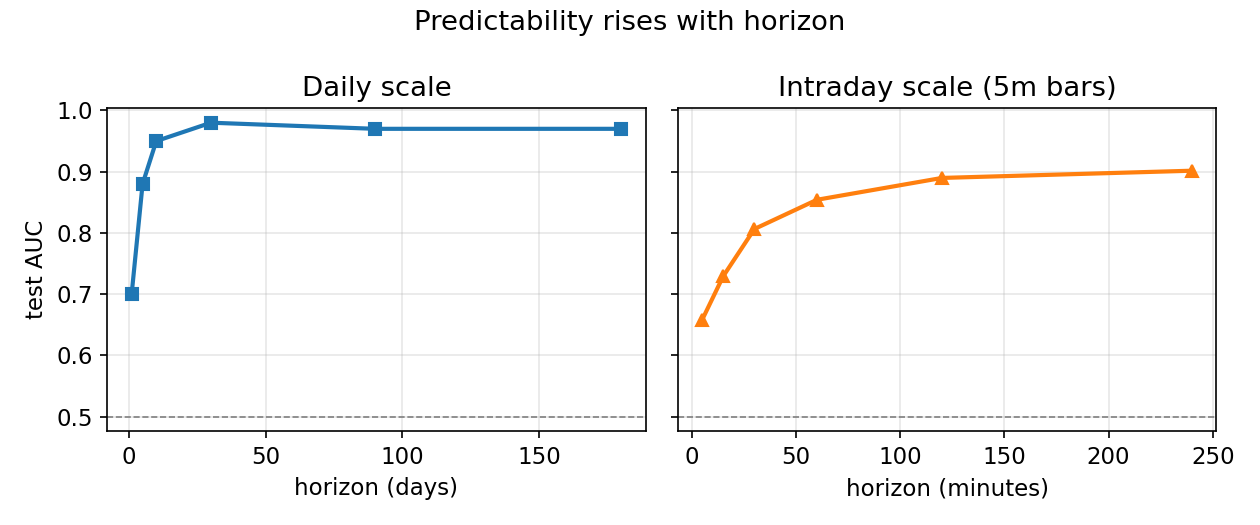
\includegraphics[width=0.92\textwidth]{figures/derivations/auc_horizon.png}
\caption{Test area under the curve by horizon. The daily scale climbs from about
$0.62$ at one day to about $0.88$ at the long horizons, and the intraday scale
climbs from about $0.67$ at five minutes to about $0.92$ at four hours.}
\label{fig:auc}
\end{figure}

\clearpage
\section{Quantile Price Bands}

The model also predicts a band of possible future returns at each horizon, not
just a volatility label, so it can express a price range. The bands are trained
with quantile regression, and this section derives why the check loss recovers a
quantile and how the monotone construction keeps the band edges from crossing.

\subsection{The Pinball Loss and the Quantile}

For a target level $\tau$ the pinball loss weights positive and negative errors
differently, which tilts the optimum toward the $\tau$ quantile. With residual
$u = y - q$ the loss is
\[
\rho_\tau(u) = \max\bigl(\tau\,u,\ (\tau-1)\,u\bigr)
= u\,\bigl(\tau - \mathbf{1}[u < 0]\bigr).
\]

We now show that the expected pinball loss is minimized at the quantile, which is
the reason this loss is used. We split the expectation at $q$ so the absolute
value opens into two integrals, then differentiate with respect to $q$ using the
Leibniz rule. The prediction $q$ appears only in the limits and in the
integrands, and the boundary terms vanish because the integrand is zero at
$u = 0$.
\begin{align*}
\mathbb{E}\bigl[\rho_\tau(Y - q)\bigr]
  &= \tau \int_{q}^{\infty} (y - q)\,f(y)\,dy
   + (1-\tau)\int_{-\infty}^{q} (q - y)\,f(y)\,dy, \\
\frac{d}{dq}\,\mathbb{E}\bigl[\rho_\tau(Y - q)\bigr]
  &= -\tau \int_{q}^{\infty} f(y)\,dy
   + (1-\tau)\int_{-\infty}^{q} f(y)\,dy \\
  &= -\tau\,\bigl(1 - F(q)\bigr) + (1-\tau)\,F(q)
   = F(q) - \tau .
\end{align*}

Setting the derivative to zero forces the cumulative probability at the optimum
to equal $\tau$, so the minimizer is exactly the $\tau$ quantile,
\[
\boxed{\,F(q^\star) = \tau \quad\Longrightarrow\quad q^\star = F^{-1}(\tau).}
\]

The subgradient used in training follows from the same expression, and it is a
constant on each side of the residual. With $e = y - q$ the derivative with
respect to the prediction $q$ is
\[
\frac{\partial \rho_\tau}{\partial q} =
\begin{cases}
-\tau, & e > 0, \\
1 - \tau, & e \le 0,
\end{cases}
\]
which is the exact branch the code writes when it forms the quantile gradient.

We confirm the theory by minimizing the empirical pinball loss over a sample of
twenty thousand standard normal draws, and the minimizer lands on the sample
quantile at every level, which is the guarantee the derivation promised.
\begin{align*}
\tau = 0.05 &\ \Rightarrow\ q^\star = -1.620, \quad \text{sample quantile} = -1.621, \\
\tau = 0.50 &\ \Rightarrow\ q^\star = -0.010, \quad \text{sample quantile} = -0.006, \\
\tau = 0.95 &\ \Rightarrow\ q^\star = +1.630, \quad \text{sample quantile} = +1.633.
\end{align*}

The shape of the loss for three levels is shown in Figure \ref{fig:pinball},
where the tilt of each arm sets which quantile the optimum finds.

\begin{figure}[H]
\centering
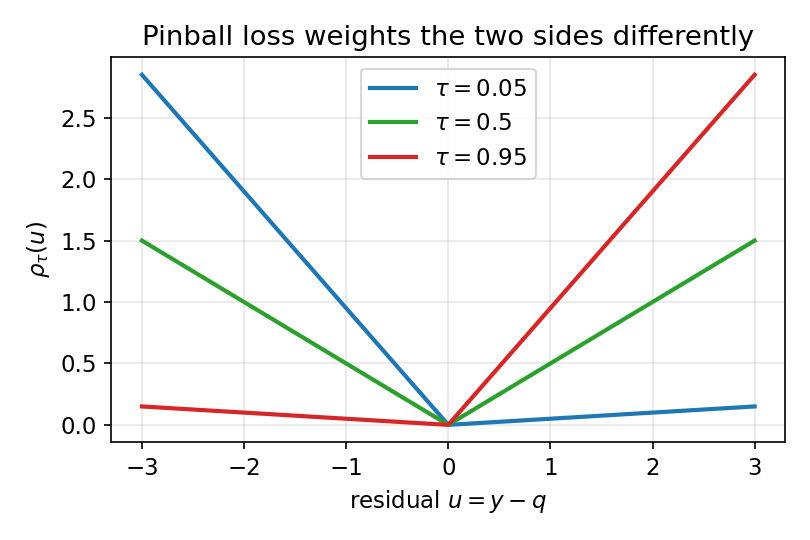
\includegraphics[width=0.66\textwidth]{figures/derivations/pinball.png}
\caption{The pinball loss for three target levels. The steeper arm penalizes the
side that must be rare, which pushes the optimum to the requested quantile.}
\label{fig:pinball}
\end{figure}

\subsection{The Monotone Non Crossing Construction}

A set of quantiles is only meaningful if the lower ones stay below the higher
ones, so we build the band to be monotone by construction rather than hoping the
optimizer keeps it ordered. The lowest quantile is a free level, and each higher
quantile adds a strictly positive increment produced by a softplus, whose output
is always positive,
\[
\text{softplus}(z) = \ln\!\left(1 + e^{z}\right) > 0 .
\]

Writing the raw head outputs as $r_{0}, r_{1}, \dots, r_{Q-1}$ the quantiles are
a running sum of these increments, which is nondecreasing because every term
added is positive,
\[
q_0 = r_0,
\qquad
q_j = r_0 + \sum_{m=1}^{j} \text{softplus}(r_m),
\qquad j = 1,\dots,Q-1 .
\]

The gradient must pass through this cumulative sum, so a change in one increment
affects every quantile at or above its index. That makes the gradient with
respect to increment $m$ a reverse cumulative sum of the upstream quantile
gradients, scaled by the softplus derivative, which is the logistic function,
\[
\boxed{\,\frac{\partial \mathcal{L}}{\partial r_m}
= \sigma(r_m)\sum_{j \ge m} \frac{\partial \mathcal{L}}{\partial q_j}.}
\]

This is exactly the reverse cumulative sum times $\sigma(\text{raw})$ that the
backward pass computes before routing the gradient into the shared trunk, so the
price bands and the volatility heads train the same representation.

\clearpage
\section{Conformal Calibration of the Bands}

Quantile heads are not guaranteed to cover their nominal rate out of sample, so
we wrap them in conformalized quantile regression, which widens the band by a
data driven amount that restores coverage with a finite sample guarantee. This
section states the score, the width, and the coverage proof.

On a held out calibration set we measure how far each true return falls outside
its predicted band, which is zero when the point is inside and positive when it
is outside. With lower and upper predictions $q_{\text{lo}}$ and $q_{\text{hi}}$
the conformity score is
\[
s_i = \max\bigl(\,q_{\text{lo}}(x_i) - y_i,\ \ y_i - q_{\text{hi}}(x_i)\,\bigr).
\]

The band widening is the empirical quantile of these scores at a level chosen so
the finite sample bound holds. For $n$ calibration points and target miscoverage
$\alpha$ the index and the widening are
\[
k = \left\lceil (1-\alpha)(n+1) \right\rceil,
\qquad
\delta = s_{(k)},
\]
where $s_{(k)}$ is the $k$ th smallest score, clamped to be nonnegative. The
calibrated band is then $[\,q_{\text{lo}} - \delta,\ q_{\text{hi}} + \delta\,]$.

The coverage guarantee rests on exchangeability of the calibration and test
points, because then the rank of the test score among the calibration scores is
uniform. A new point is covered exactly when its score does not exceed $\delta$,
so its miscoverage probability is the chance that its score lands above the $k$
th order statistic,
\[
\mathbb{P}\bigl(s_{n+1} > s_{(k)}\bigr) = \frac{n + 1 - k}{n + 1}
\le \alpha .
\]

Taking the complement gives the finite sample coverage bound that the
calibration targets, and it holds for any underlying model,
\[
\boxed{\,\mathbb{P}\Bigl(Y_{n+1} \in \bigl[\,q_{\text{lo}} - \delta,\ q_{\text{hi}} + \delta\,\bigr]\Bigr)
\ge 1 - \alpha .}
\]
We demonstrate the widening on a deliberately narrow band. Starting from a band
that covers only $0.683$ of a normal sample, five hundred calibration scores set
the widening to $\delta = 0.669$ at the index $k = 451$, and the calibrated band
then covers $0.907$ of fresh data against the target of $0.90$. Figure
\ref{fig:conformal} shows the distribution of the scores with the chosen
widening marked.

\begin{figure}[H]
\centering
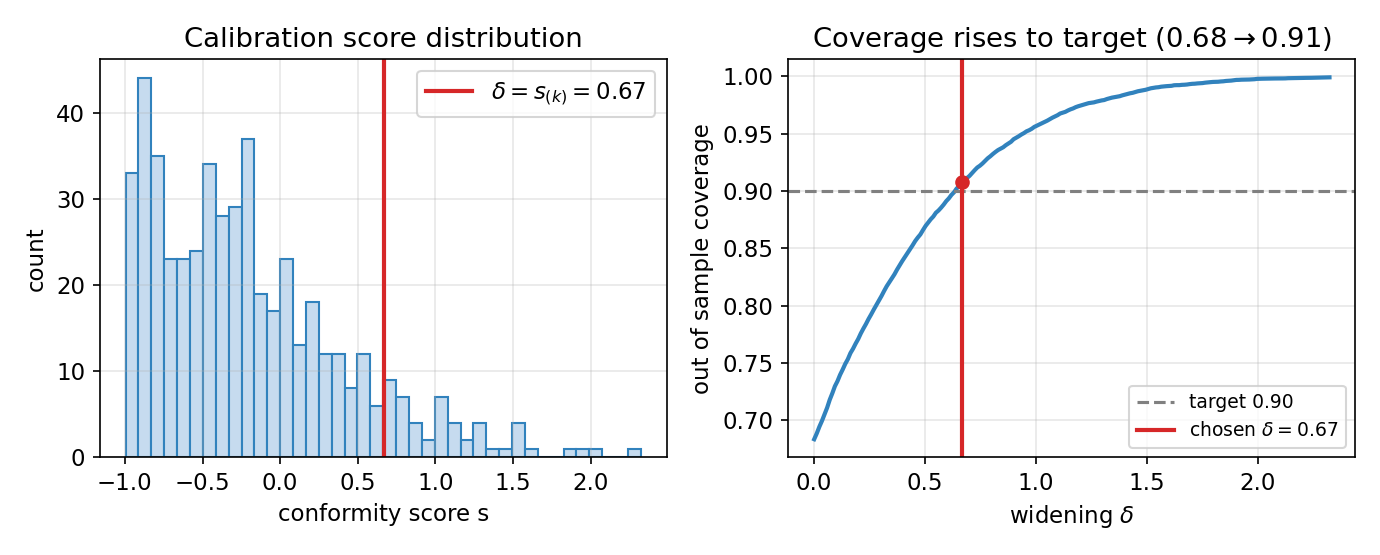
\includegraphics[width=0.92\textwidth]{figures/derivations/conformal.png}
\caption{Left, the distribution of conformity scores on the calibration set with
the order statistic $\delta = s_{(k)}$ marked. Right, out of sample coverage as a
function of the widening $\delta$. Coverage increases monotonically and the
chosen $\delta$ lands it on the target, lifting coverage from $0.68$ to $0.91$.}
\label{fig:conformal}
\end{figure}

The widening acts on the band edges only, so it restores coverage without moving
the center of the forecast. Figure \ref{fig:conformalbands} shows the same
calibration on the data, with the original narrow band, the widened band, and the
points that each one covers.

\begin{figure}[H]
\centering
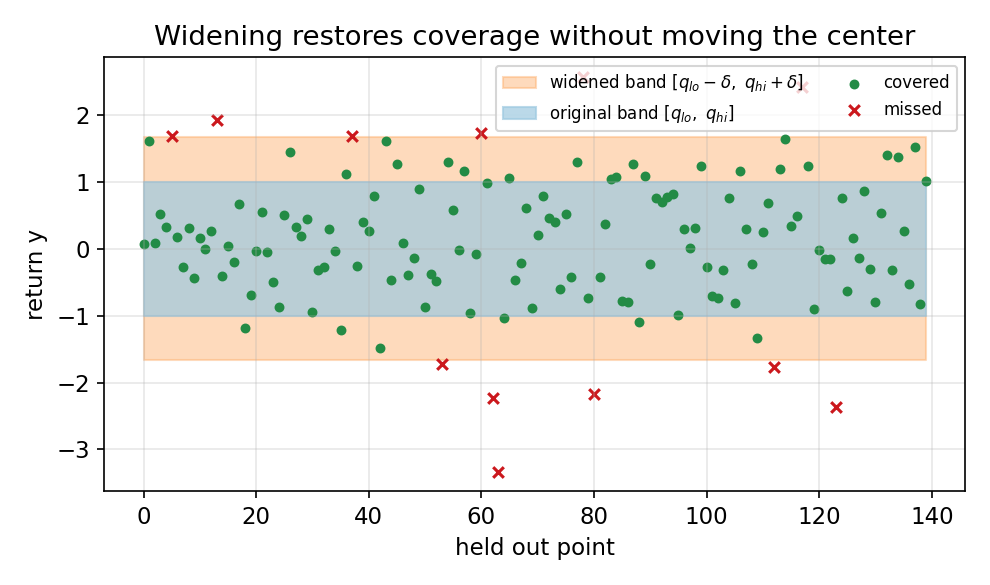
\includegraphics[width=0.72\textwidth]{figures/derivations/conformal_bands.png}
\caption{The original band in blue covers too few points, and the conformal
widening in orange extends the edges by $\delta$ so the covered fraction reaches
the nominal level. The center of the band does not move, only its width.}
\label{fig:conformalbands}
\end{figure}
The example price cone reported at the end of a run turns these return quantiles
into prices through $P = P_0\,e^{q}$, because the model works in log return space
where the bands are symmetric and additive.

The grade of the cone, meaning how fast it widens with the horizon, is set by
integrating the variance under the volatility curve rather than by any single
volatility. Returns over disjoint days are close to uncorrelated, so variances
add across time, and the variance of the cumulative return to horizon $h$ is the
area under the instantaneous variance curve. The half width of the band scales
with the square root of that integral,
\[
\sigma_{\text{cum}}(h) = \sqrt{\int_0^{h} \sigma^2(\tau)\, d\tau}
\ \approx\ \sqrt{\sum_{k=1}^{h} \sigma_k^2},
\]
where $\sigma_k$ is the measured volatility on day $k$ taken from the term
structure. Because the measured volatility rises with the horizon the integrated
variance grows faster than a flat volatility would predict, so the cone is
steeper and it matches the grade of the data. A flat one day volatility is the
special case where $\sigma(\tau)$ is constant, which understates the area and
flattens the cone.

Figure \ref{fig:cone} shows the cone interacting with the data projection. We
build the band from the measured volatility term structure using the normal
quantiles, and we project the data by simulating four thousand price paths under
the same rising volatility schedule. The shaded model cone and the empirical
quantiles of the simulated paths track each other closely, and the fraction of
paths that finish inside the five to ninety five band is $0.901$, which matches
the nominal ninety percent. Working the one hundred eighty day edges through
$P = 100\,e^{q}$ gives
\begin{align*}
\text{5th } &\$66.36 \ (\text{data } \$66.32), &
\text{25th } &\$84.52 \ (\text{data } \$84.25), \\
\text{50th } &\$100.00 \ (\text{data } \$100.67), &
\text{75th } &\$118.32 \ (\text{data } \$119.74), \\
\text{95th } &\$150.70 \ (\text{data } \$150.32). & &
\end{align*}

\begin{figure}[H]
\centering
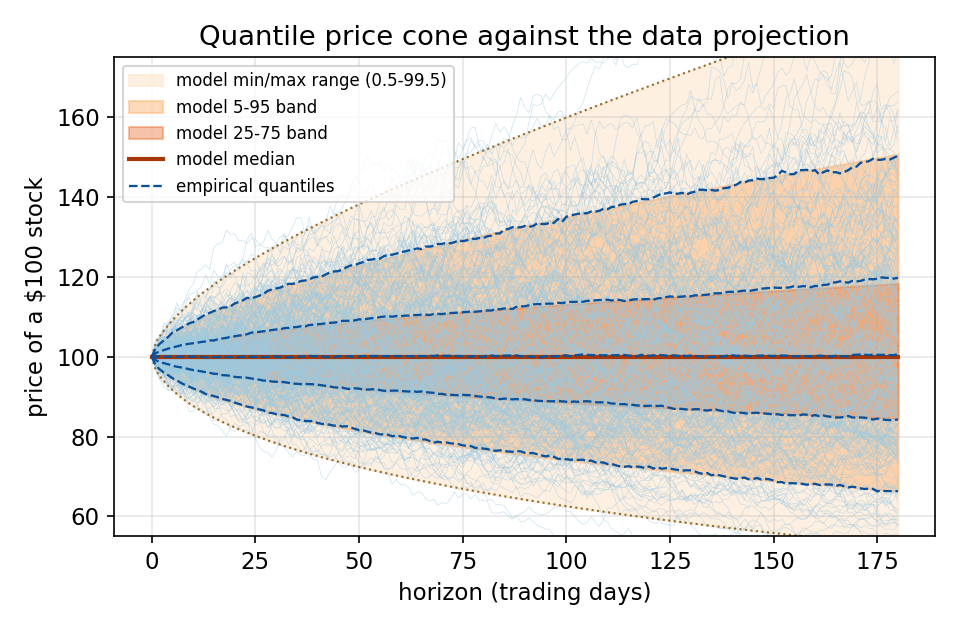
\includegraphics[width=0.82\textwidth]{figures/derivations/price_cone.png}
\caption{The quantile price cone against the data projection. The light lines are
simulated price paths, the shaded regions are the model bands, and the dashed
lines are the empirical quantiles of the paths. The cone widens as the square
root of the integrated variance under the volatility curve and contains the
paths at the nominal rate.}
\label{fig:cone}
\end{figure}

\clearpage
\section{Evaluation by the Area Under the ROC Curve}

We judge every horizon by the area under the receiver operating characteristic
curve, because it measures ranking quality and is invariant to the threshold and
to class imbalance. The curve plots the true positive rate against the false
positive rate as the decision threshold sweeps, and the area under it has a
probabilistic meaning that leads to a fast estimator.

The area is the integral of the true positive rate over the false positive rate,
and that integral equals the probability that a random positive is scored above
a random negative,
\[
\mathrm{AUC} = \int_0^1 \mathrm{TPR}\,d(\mathrm{FPR})
= \mathbb{P}\bigl(S^{+} > S^{-}\bigr).
\]

Estimating that probability by counting ordered pairs would cost a quadratic
number of comparisons, so we use the Mann Whitney identity, which reads the same
count off the ranks. Sorting all scores and summing the ranks of the positives
gives the estimator the code implements,
\[
\boxed{\,\widehat{\mathrm{AUC}}
= \frac{R^{+} - \tfrac{1}{2}\,n_{+}\,(n_{+}+1)}{n_{+}\,n_{-}},}
\]
where $R^{+}$ is the sum of the ranks of the positive examples and $n_{+}$ and
$n_{-}$ are the counts of positives and negatives. The subtracted term removes
the ranks that positives contribute among themselves, so what remains counts
only the positive over negative wins.

We check the identity on a labeled sample of forty scores. The rank based formula
and a direct count of ordered pairs give the same value, which confirms the two
views agree,
\[
\widehat{\mathrm{AUC}}_{\text{ranks}} = 0.6522
= \widehat{\mathrm{AUC}}_{\text{pairs}} = 0.6522 .
\]

The corresponding curve is shown in Figure \ref{fig:roc}, where the area above
the diagonal is the reported score.

\begin{figure}[H]
\centering
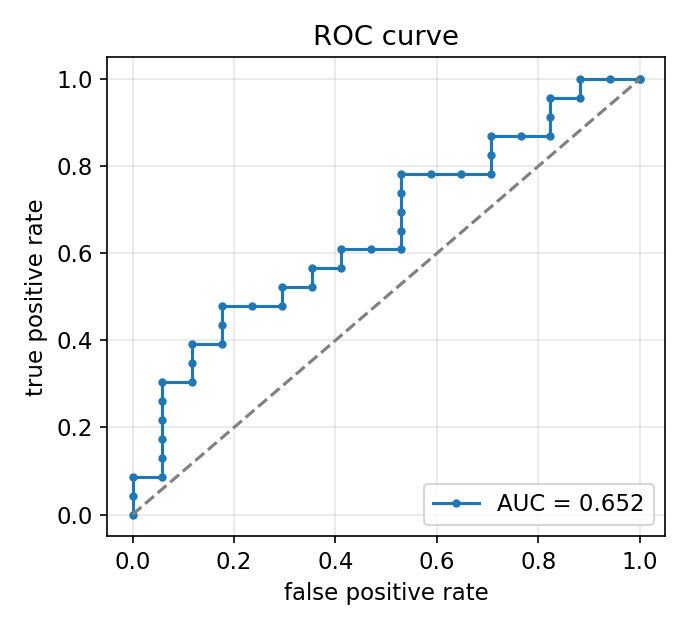
\includegraphics[width=0.5\textwidth]{figures/derivations/roc.png}
\caption{An ROC curve for the worked sample. The diagonal is the chance line, and
the area under the curve equals the rank based estimate of $0.652$.}
\label{fig:roc}
\end{figure}

\clearpage
\section{The Ensemble}

The final prediction blends the cross sectional volatility model with the multi
scale term structure model, because they read different views of the same event
and their errors are partly independent. Both output a probability that the next
horizon volatility is above the cross sectional median, so a convex combination
is a valid probability,
\[
p_{\text{ens}} = a\,p_{\text{ucn}} + (1 - a)\,p_{\text{ms}},
\qquad a \in [0, 1].
\]

The blend weight is chosen to maximize validation area under the curve over a
grid, which picks the mix that ranks best out of sample,
\[
\boxed{\,a^\star = \arg\max_{a \in [0,1]}
\ \mathrm{AUC}\bigl(y,\ a\,p_{\text{ucn}} + (1-a)\,p_{\text{ms}}\bigr).}
\]

When only one model has inputs available the search degenerates to that model
alone, so the ensemble always reduces gracefully to whichever component is
present.

\clearpage
\section{Summary of the Pipeline}

The project chains the pieces above into one estimator. We compute log returns
and forward realized volatility, rank the volatility within each date to form
market neutral labels, standardize the features on training rows, and keep the
features with the most mutual information with the target. The unified network
combines a logistic branch, a Gaussian naive Bayes branch, a rectified network,
a sentiment branch, and an LSTM branch under a softmax meta layer, and it is
trained by Adam with cross entropy. The multi scale model adds six window LSTM
branches linked by their drift, six volatility heads coupled by a curvature
penalty, and quantile heads that produce conformally calibrated price bands. We
score every horizon by the area under the ROC curve and blend the two models
into a single calibrated probability. Every equation in this document is the one
the code evaluates, so the statistics and the software describe the same model.

\end{document}
